\documentclass{standalone}
\usepackage{tikz}
\tikzset{block/.style = {draw, fill=white, very thick, rectangle, minimum height=1cm, minimum width=2cm},  
         square/.style = {draw, fill=white, very thick, rectangle, minimum height=1cm, minimum width=1cm},
         sum/.style= {draw, fill=white, very thick, circle, node distance=0.5cm}} 
\begin{document}
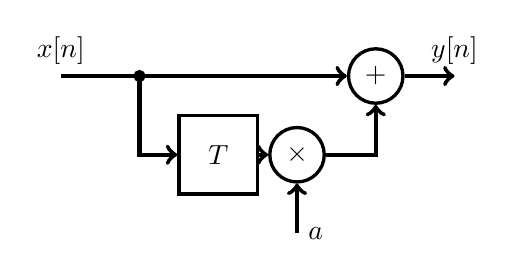
\begin{tikzpicture}[scale=2]
    \node[sum](+)at(2,0){$+$};
        \draw[->,ultra thick](0,0)node[above]{$x[n]$}--(+.180);
        \filldraw[black](0.5,0)circle(1pt);

        \node[square](t)at(1,-0.5){$T$};
        \draw[->,ultra thick](0.5,0)--(0.5,-0.5)--(t.180);

        \node[sum](x)at(1.5,-0.5){$\times$};
        \draw[->,ultra thick](t.0)--(x.180);
        \draw[->,ultra thick](1.5,-1)node[right]{$a$}--(x.270);

        \draw[->,ultra thick](x.0)--(2,-0.5)--(+.270);
        \draw[->,ultra thick](+.0)--(2.5,0)node[above]{$y[n]$};
\end{tikzpicture}
\end{document}